\documentclass[crop=true,tikz,border=1pt,varwidth=8in]{standalone}

%\makeatletter
%%%%%%%%%%%%%%%%%
\PassOptionsToPackage{force}{filehook}
\usepackage{tikz}
\usetikzlibrary{shapes,arrows}
\usetikzlibrary{positioning}
\tikzstyle{cloud} = [draw, ellipse,fill=red!20, node distance=0.87cm,
minimum height=2em]
\tikzstyle{line} = [draw, -latex']
\usetikzlibrary{shapes.symbols,shapes.callouts,patterns}
\usetikzlibrary{calc}


\begin{document}
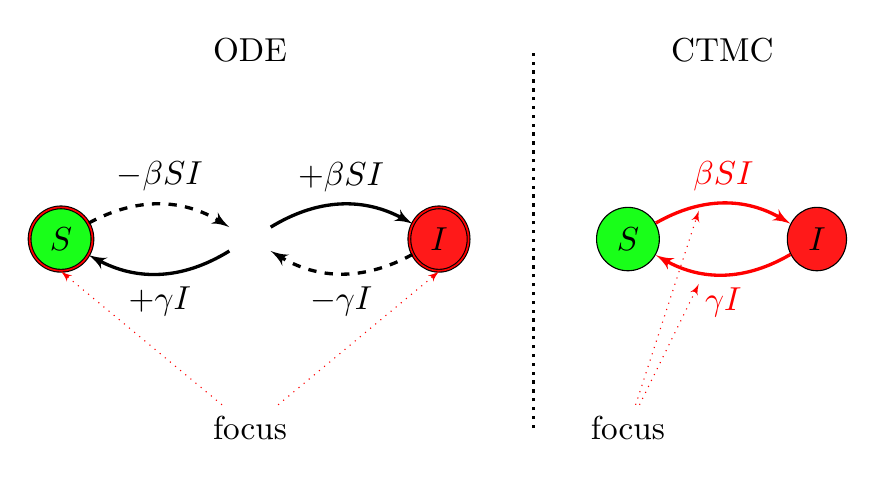
\begin{tikzpicture}[auto,
    scale=1.2, every node/.style={transform shape},
    cloud/.style={minimum width={width("N-1")+2pt},
    draw, ellipse,fill=red!20}]
    \node[cloud, fill=green!90, double=red] (S) at (0,0) {$S$};
    \node[cloud, draw=none, fill=white] (h4) at (2,0) {};
    \node[cloud, fill=red!90, double=red] (I) at (4,0) {$I$};
    \node[cloud, fill=green!90] (S2) at (6,0) {$S$};
    \node[cloud, fill=red!90] (I2) at (8,0) {$I$};
    %% Flows (ODE)
    \path [line, bend left, very thick, dashed] (S) to node [midway, above] (TextNode) {$-\beta SI$} (h4);
    \path [line, bend left, very thick] (h4) to node [midway, below] (TextNode) {$+\gamma I$} (S);
    \path [line, bend left, very thick] (h4) to node [midway, above] (TextNode) {$+\beta SI$} (I);
    \path [line, bend left, very thick, dashed] (I) to node [midway, below] (TextNode) {$-\gamma I$} (h4);
    %% Flows (CTMC)
    \path [line, bend left, very thick, red] (S2) to node [midway, above] (TextNode) {$\beta SI$} (I2);
    \path [line, bend left, very thick, red] (I2) to node [midway, below] (TextNode) {$\gamma I$} (S2);
    %%
    \draw[very thick, dotted] (5,-2) -- (5,2);
    %%
    \node[style=rectangle] at (2,2) {ODE};
    \node[style=rectangle] at (7,2) {CTMC};
    %%
    \node[style=rectangle] (fODE) at (2,-2) {focus};
    \path [line, dotted,red] (fODE) to  (S.south);
    \path [line, dotted,red] (fODE) to  (I.south);
    \node[style=rectangle] (fCTMC) at (6,-2) {focus};
    \path [line, dotted,red] (fCTMC) to (6.75,0.3);
    \path [line, dotted,red] (fCTMC) to  (6.75,-0.475);
\end{tikzpicture}        
\end{document}
